%%
%% Chapter: 6
%%
\cleardoublepage  %  flush all material and start a new page, start new odd numbered page. 
\chapter{Appendices}
\label{cha:Appendices}      %% No special characters, no space 
%\addcontentsline{toc}{chapter}{Appendices}

This section contains all
\begin{itemize}
	\item questionnaires,
	\item interview transcripts,
	\item pilot reports,
	\item detailed tables, etc.
\end{itemize}

\paragraph{Demonstration of abbreviations}
Define a glossary entry in file \textit{Acronyms.tex}:
\newline
\verb!\newacronym{utc}{UTC}{Coordinated Universal Time}!
\newline
Use a glossary entry: \verb! \gls{utc} !
\newline
This \LaTeX code \\

\verb*|\gls{utc} is 3 hours behind \gls{adt}.| \\

will produce this: \\

\gls{utc} is 3 hours behind \gls{adt}.\\

At the first time usage, the abbreviation is mentioned in brackets.

With the second usage of an abbreviation, the abbreviated term itself is not shown any more:
\gls{utc} is still 3 hours behind \gls{adt}.\\

\paragraph{Demonstration of a stacked bar chart}
Figure \ref{fig:StackedBarChart} shows an example of a stacked bar chart generated with tikzpicture (pgfplots package).

\begin{figure}
	\centering
	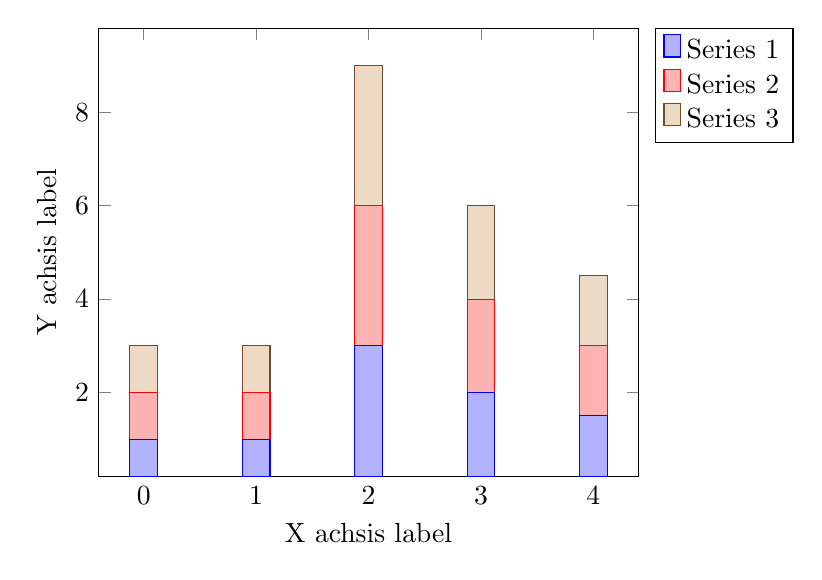
\begin{tikzpicture}
		\begin{axis}[ybar stacked, 
			xlabel=X achsis label, 
			ylabel=Y achsis label,
			legend cell align=left,
			legend pos=outer north east]
			\addplot coordinates 
			{(0,1) (1,1) (2,3) (3,2) (4,1.5)};
			\addplot coordinates
			{(0,1) (1,1) (2,3) (3,2) (4,1.5)};
			\addplot coordinates
			{(0,1) (1,1) (2,3) (3,2) (4,1.5)};
			\legend{Series 1, Series 2, Series 3}
		\end{axis}
	\end{tikzpicture}
	\caption{\label{fig:StackedBarChart}Title to the bar chart}
\end{figure}

\paragraph{Demonstration of a pie chart}
Figure \ref{fig:PieChart} shows an example of a pie chart generated with tikzpicture (pgf-pie package).

\begin{figure}
	\centering
	\begin{tikzpicture}
		\pie [rotate = 180]
		{
			62/Category A,
			32/Category B, 
			6/Other
		}
		\end{tikzpicture}
	\caption{\label{fig:PieChart}Title to the pie chart}
\end{figure}

\paragraph{Demonstration of a line chart}
Figure \ref{fig:LineChart} shows an example of a simple chart generated with tikzpicture (packages pgfplots and pgfplotstable). 
The regression is also rendered and the formula $ y(x_i) = a \cdot x_i + b$ displayed. The values a and b will be stored globally.

\begin{figure}
	\centering
	\begin{tikzpicture}
		\begin{axis}[legend pos=outer north east]
			\addplot table[row sep=\\] {% plot X versus Y. This is original data.
				X Y\\
				1 1 \\
				2 4\\
				3 9\\
				4 16\\
				5 25\\
				6 36\\
			};
			\addplot table[row sep=\\,
			y={create col/linear regression={y=Y}}] % compute a linear regression from the input table
			{
				X Y\\
				1 1 \\
				2 4\\
				3 9\\
				4 16\\
				5 25\\
				6 36\\
			};
			\addlegendentry{$y(x)$}
			\addlegendentry{%
				$\pgfmathprintnumber{\pgfplotstableregressiona} \cdot x
				\pgfmathprintnumber[print sign]{\pgfplotstableregressionb}$}
		\end{axis}

	\end{tikzpicture}
	\caption{\label{fig:LineChart}Title to the line chart}
\end{figure}

\paragraph{Demonstration of a table}
Table \ref{tbl:Salinity-EC} shows an example of a table.

\begin{table}
	\begin{center}
		\caption{\label{tbl:Salinity-EC}Conductivity values measured for defined salinity values}
		\begin{tabular}{cc}
			\hline \\
			Salinity [g/L]	& 	Electrical Conductivity [mS/cm]\\    
			\\
			\hline \\
			40	&	63,3	\\
			35	&	55,1	\\
			30	&	47,2	\\
			25	&	40,4	\\
			20	&	32,9	\\
			15	&	25,5	\\
			10	&	17,53	\\
			5	&	9,39	\\
			\hline \\
		\end{tabular}  
	\end{center}
\end{table}

\paragraph{Demonstration of including a PDF}
Figure \ref{fig:GF543kv} shows an example of a PDF. The section displayed is of a particular page from the PDF and is cropped in size.
\begin{figure}
	\centering
	\includegraphics[width=0.9\textwidth,page=6, trim = 25mm 172mm 25mm 45mm, clip]{600-Appendices/Datasheet_GF_543}
	\caption{GF ball valve 543 kv-characteristic}
	\label{fig:GF543kv}
\end{figure}

\paragraph{Demonstration of including a JPG with labels}
Figure \ref{fig:HeatExchanger} shows an example of a JPG that has some labels applied.

\begin{figure}
	\centering
	\setlength {\unitlength}{0.1\textwidth}
	\begin{picture} (10,7)(0,0)
		\setlength\fboxsep{1 mm}
		\put(0,0){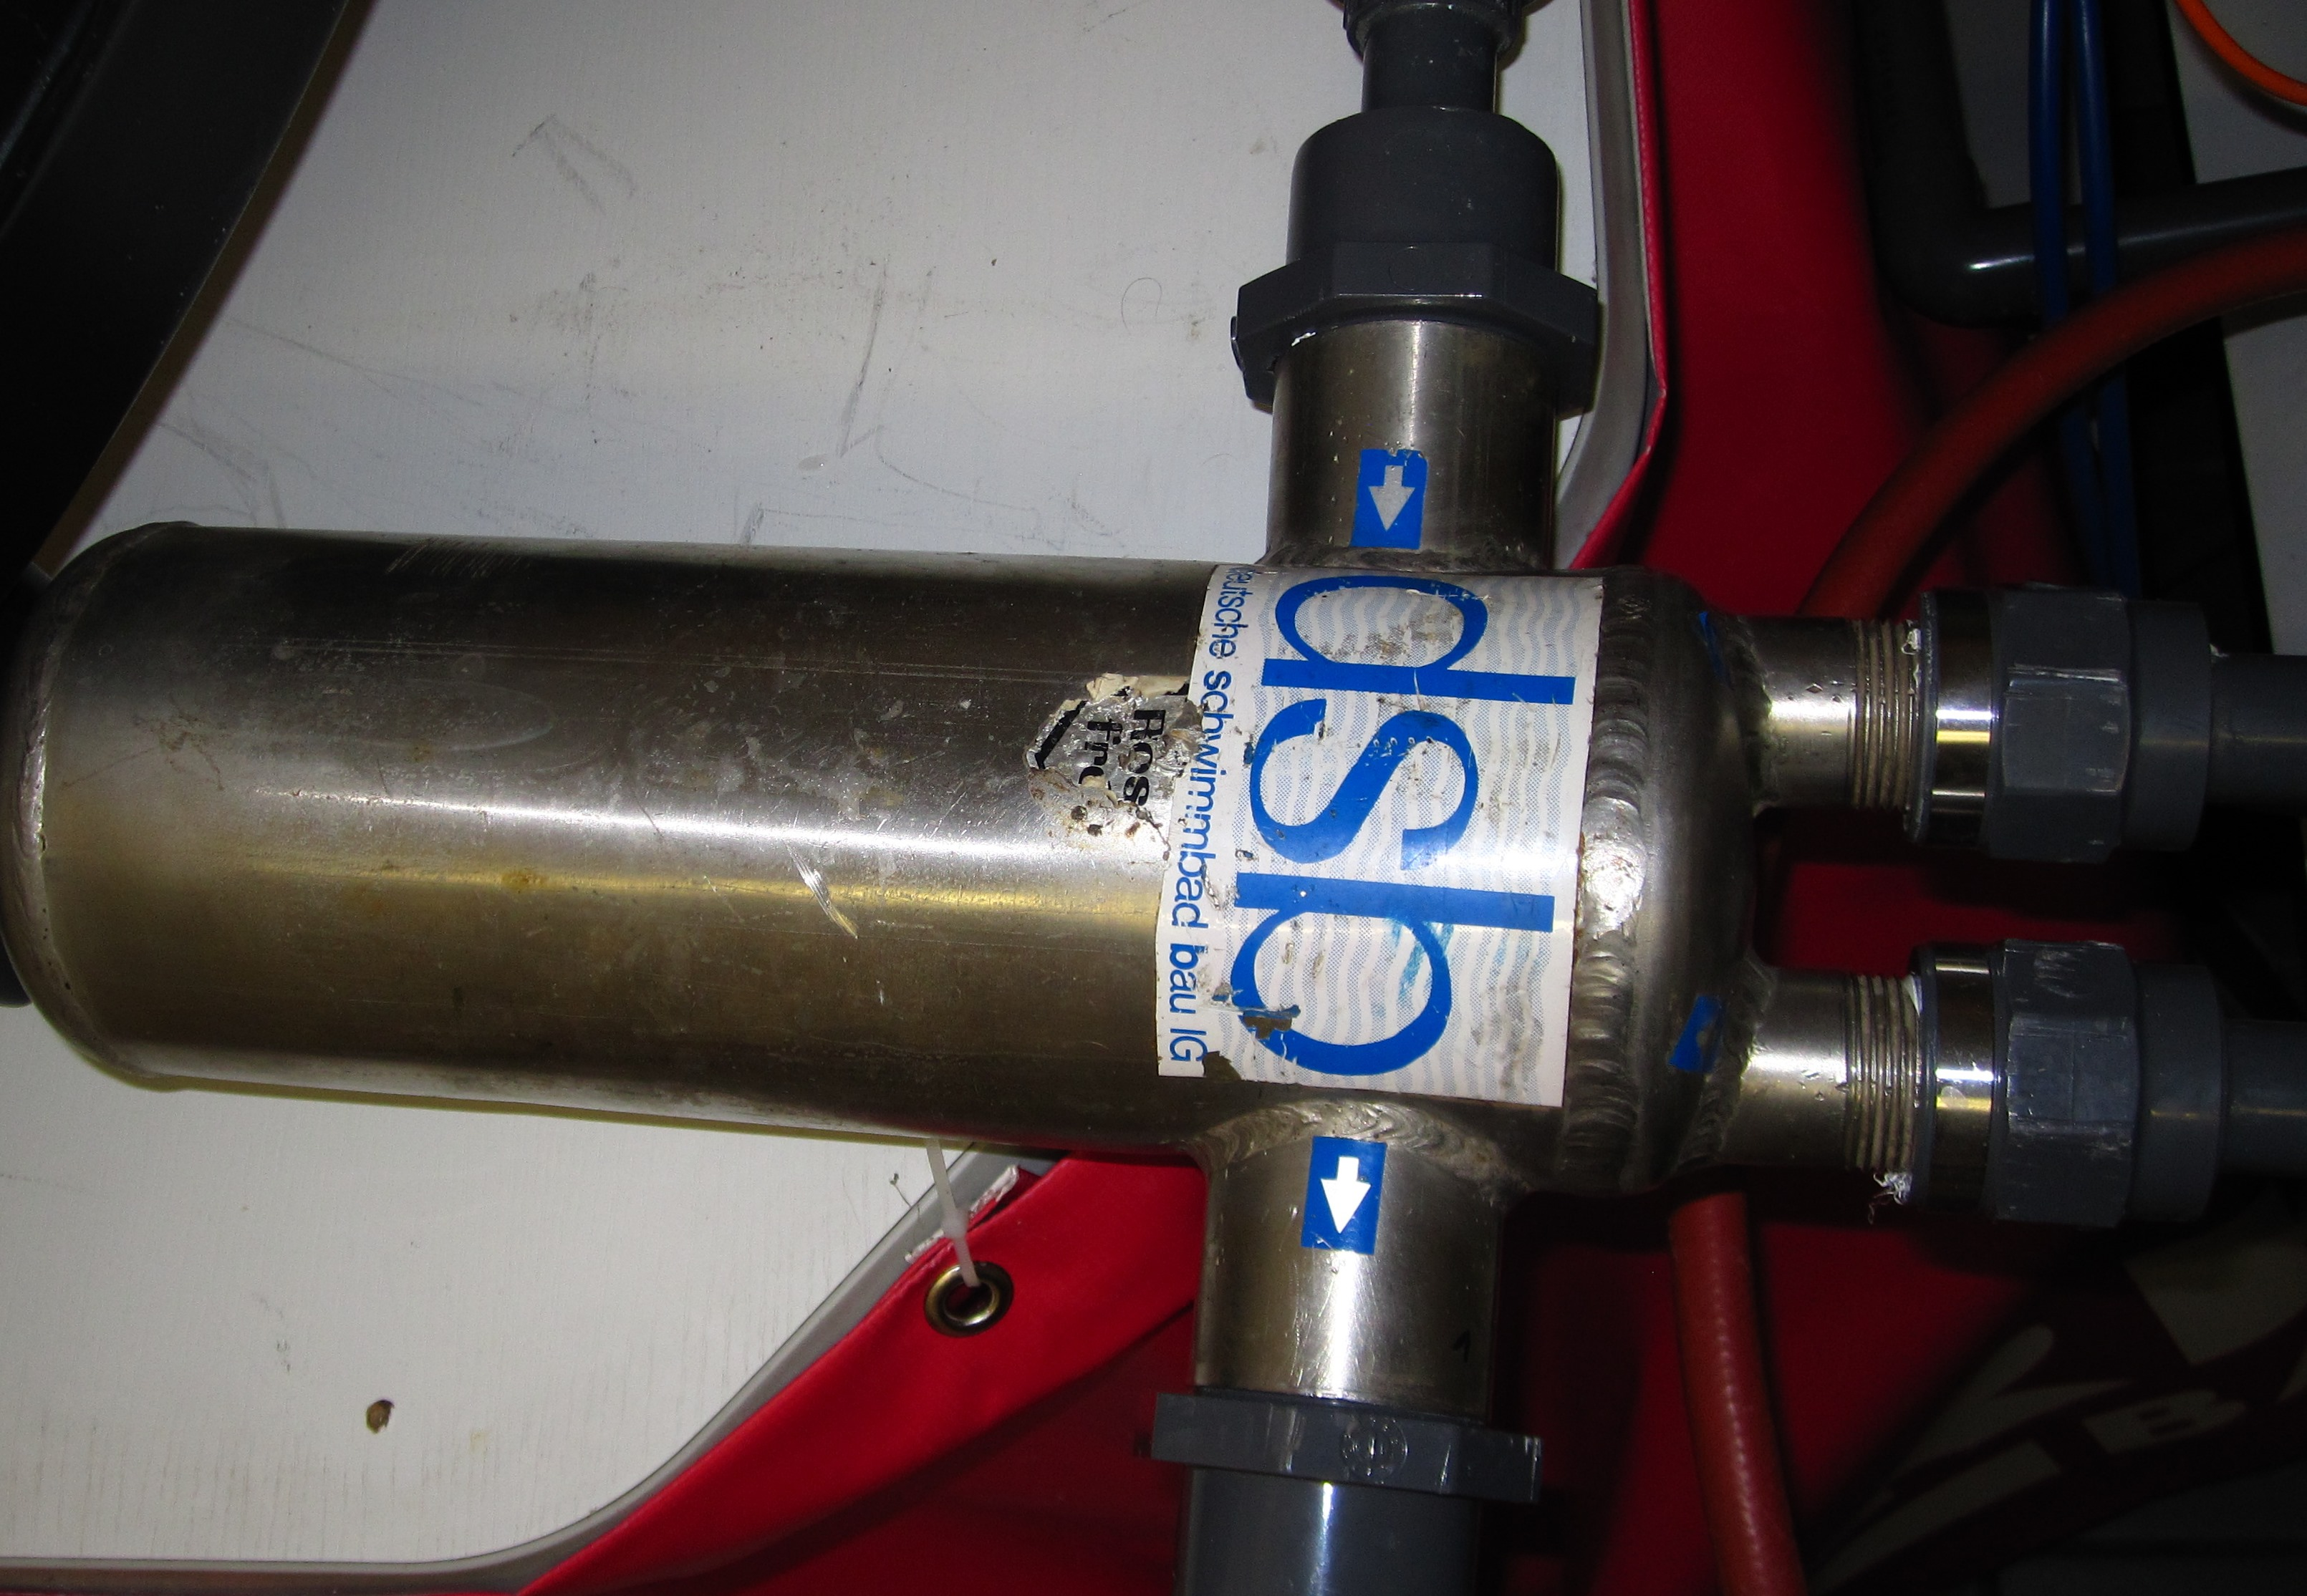
\includegraphics[width=\textwidth]{600-Appendices/Heat_Exchanger.jpg}}
		\put(4,5){\colorbox{red!20}{\framebox[1.1\width]{Concentrate in}}}
		\put(3,1){\colorbox{red!20}{\framebox[1.1\width]{Concentrate out}}}
		\put(7,4.5){\colorbox{blue!20}{\framebox[1.1\width]{From exchanger}}}
		\put(7,1.5){\colorbox{blue!20}{\framebox[1.1\width]{To exchanger}}}
	\end{picture}              
	\caption{Heat exchanger with flow of media}
	\label{fig:HeatExchanger}
\end{figure}

\paragraph{Demonstration of citation}
Table \ref{tbl:CitationStyles} shows some different options on how to cite a source.

\begin{table}
	\begin{center}
		\caption{\label{tbl:CitationStyles}Some styles to citation}
		\begin{tabular}{lll}
			\hline \\
			Command & 	Output	& Description \\
			\\
			\hline \\
			\verb! \cite{ref} ! & \cite{Monippally2010} & Textual\\
			\verb! \citep[page]{ref} ! & \citep[p. 20]{Monippally2010} & Parenthetical citation\\
			\verb! \citeauthor{ref} ! & \citeauthor{Monippally2010} & Name of author\\
			\verb! \citeyear{ref} ! & \citeyear{Monippally2010} & Year of publication\\
			\hline \\
		\end{tabular}  
	\end{center}
\end{table}

\paragraph{Demonstration of formulas}
Formula \ref{Population} shows the geometrical projection formula for population growth.

The parameters description is done using the macro \textit{conditions}, defined at the beginning of main.tex.
\begin{equation}\label{Population}
P_f=P_0(1+\frac{i}{100})^t
\end{equation}
where:
\begin{conditions}
	P_f	&	Future population \\
	P_0	&	Current population \\
	i	&	Growth rate in \% \\   
	t	&	Time in years
\end{conditions}

The Hazen-Williams formula expressed in metric units as seen in \ref{Hazen-William}
\begin{equation}\label{Hazen-William}
H[m]= \Big( \frac{6.78 L}{d^{1.165}} \Big) \Big({\frac{V}{C}} \Big)^{1.85}
\end{equation}
where:
\begin{conditions}
	H	&	Headloss \\
	L	&	Length of pipe\\
	d	&	Internal diameter of pipe \\   
	V	&	Flow \\
	C	&	Coefficient
\end{conditions}

\paragraph{Demontration of links}
Use \verb!\href{URL}{DESCRIPTION}! to add a link with description.
Use \verb!\url{URL}! to add a link without a description.

The Water Research \& Development Centre's website: \url{https://nduwrdc.org}